
\documentclass[dvipdfmx]{standalone}
\usepackage[T1]{fontenc}
\usepackage{newtxtext, newtxmath}

\usepackage{tikz}
\usetikzlibrary{positioning}

\begin{document}
  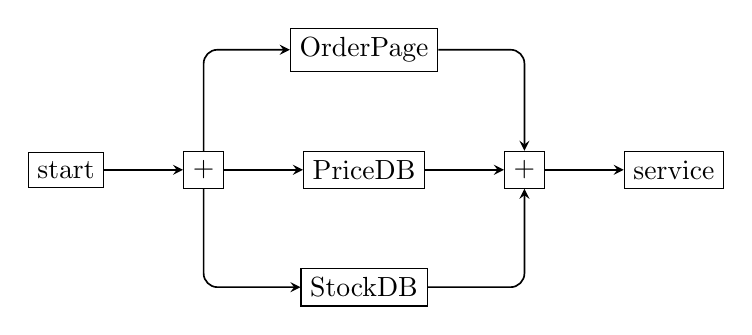
\begin{tikzpicture}
    \tikzset{myarrow/.style={>=stealth, semithick, rounded corners=5pt}}

    \draw node[draw] (start) {start};
    \draw node[draw, right=of start] (split) {+};
    \draw node[draw, right=of split] (pricedb) {PriceDB};
    \draw node[draw, above=of pricedb] (orderpage) {OrderPage};
    \draw node[draw, below=of pricedb] (stockdb) {StockDB};
    \draw node[draw, right=of pricedb] (join) {+};
    \draw node[draw, right=of join] (service) {service};

    \draw[->, myarrow] (start) -- (split);
    \draw[->, myarrow] (split) -- (pricedb);
    \draw[->, myarrow] (split) |- (orderpage);
    \draw[->, myarrow] (split) |- (stockdb);
    \draw[->, myarrow] (pricedb) -- (join);
    \draw[->, myarrow] (orderpage) -| (join);
    \draw[->, myarrow] (stockdb) -| (join);
    \draw[->, myarrow] (join) -- (service);
  \end{tikzpicture}
\end{document}
